\documentclass[]{report}

\usepackage[a4paper]{geometry}

\usepackage{parskip}
\usepackage{amsmath}
\usepackage{physics}
\usepackage{amssymb}
\usepackage[hidelinks]{hyperref}
\usepackage{dirtytalk}

\usepackage{fnpct}

\usepackage{tikz}

\renewcommand{\emph}{\textbf}

\newcommand{\resources}{\mathcal{R}}
\newcommand{\resourcesg}{\mathcal{R}_g}
\newcommand{\resourcesr}{\mathcal{R}_r}
\newcommand{\resourcesn}{\mathcal{R}_n}
\newcommand{\resourcesm}{\mathcal{R}_m}

\newcommand{\componentsr}{\mathcal{C}_r}

\newcommand{\groups}{\mathcal{G}}
\newcommand{\groupsr}{\mathcal{G}_r}

\newcommand{\markets}{\mathcal{M}}
\newcommand{\marketsg}{\mathcal{M}_g}
\newcommand{\marketsr}{\mathcal{M}_r}

\newcommand{\timesteps}{\mathcal{T}}

\newcommand{\outputs}{\mathcal{O}}
\newcommand{\outputse}{\mathcal{O}_e}
\newcommand{\inputs}{\mathcal{I}}

\newcommand{\sign}{\sigma}

\newcommand{\pmax}{\overline{P}}

\newcommand{\soc}{q}
\newcommand{\socinit}{Q_0}
\newcommand{\socmax}{\overline{Q}}
\newcommand{\socmin}{\underbar{Q}}

\newcommand{\pdmax}{\overline{P}^\mathrm{D}}
\newcommand{\pcmax}{\overline{P}^\mathrm{C}}

\newcommand{\ub}[1]{\overline{#1}}
\newcommand{\lb}[1]{\underline{#1}}

\newcommand{\aup}{a^{\uparrow}}
\newcommand{\adown}{a^{\downarrow}}
\newcommand{\rup}{r^{\uparrow}}
\newcommand{\rdown}{r^{\downarrow}}

\newcommand{\dfup}{\Delta f^\uparrow}
\newcommand{\dfdown}{\Delta f^\downarrow}

\newcommand{\cfcrnr}{C^\text{FCR-N,R}}

\newcommand{\cupa}{C^{A\uparrow}}
\newcommand{\cdowna}{C^{A\downarrow}}

\let\oldforall\forall
\renewcommand{\forall}{\; \oldforall \: }


\begin{document}

\vspace*{5cm}

\begin{center}
    {\LARGE  AggregatorX}
\end{center}

\newpage

\tableofcontents

\chapter{Mathematical description}

\section{Basic concepts}
The primary motivation for the framework is to provide an extensible tool for analyzing flexible distributed energy resources and their interaction with energy and balancing markets. The main task of the framework is to set up and solve an optimization problem that optimizes the net profit for a given portfolio of flexible energy resources.

The basic concept of the framework is a set of components (further described in the coming sections) that can exchange energy. At the core of each component is conservation of energy which also includes storage and loss/generation to/from surroundings. Depending on the system of interest, the user may connect various components from a library and connect them appropriately to represent the system. Custom components may also readily be defined if the current library is insufficient. Each component, depending on the the type, will add \emph{parameters}, \emph{variables}, \emph{constraints} or \emph{objective function terms} to the optimization problem to be solved.

\begin{figure}    
    \centering
    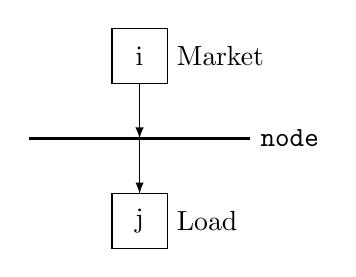
\begin{tikzpicture}[scale = 0.7]
        \draw (-.5,0) rectangle node {j} (.5,1);
        \node at (.5,.5) [anchor = west] {Load};
        \draw[-latex] (0,2) -- (0,1);
        \draw[very thick, font = \ttfamily] (-2,2) -- (2,2) node [right] {node};
        \draw[-latex] (0,3) -- (0,2);
        \draw (-.5,3) rectangle node {i} (.5,4);
        \node at (.5,3.5) [anchor = west] {Market};
    \end{tikzpicture}
    \caption{A minimum working system consisting of a market, a node and a load. Each arrow represents a unidirectional connection/power flow between the components.}
    \label{fig:marketload}
\end{figure}

Let us first look at the conceptual ideas of the framework through a series of simple example systems. The overall system consists of \emph{components} that transmit energy through \emph{connections} and the entire system is described by these components and their connections. Each specific component belongs to one of a few general component \textit{categories} that will be introduced as we proceed. Two of these are \emph{markets} and (flexible) \emph{resources}. A minimal working system definition is illustrated in figure \ref{fig:marketload}. A market represents a component where energy may be purchased or sold at a price. Resources can be be classified as either load/generation (sources or sinks of energy) or storage units. These markets and resources are connected through \emph{nodes} which represents a lossless transmitter of energy between the various components (one can think of this as a system bus or bus bar). The node only introduces the constraint that the power flowing in to the node must be equal to the power flowing out of the node. Different types of loads may be defined, e.g require a minimum power in certain time intervals.

The model can be extended with more resources. Figure \ref{fig:marketloadbatterygen} illustrates a system where we have added a generation unit (e.g. a photovoltaic (PV) unit) and a battery. The PV generation resource will typically provide a generation profile which is the power flowing into to node in each time step. The battery can store energy and will typically have several physical restrictions, e.g maximum charge and discharge rates. Note that connections are uni-directional so if energy can flow both ways in the battery, two connections are needed.

\begin{figure}
    \centering
    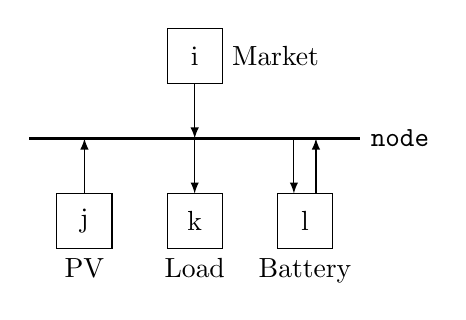
\begin{tikzpicture}[scale=0.7]
        %PV
        \draw (-2.5,0) rectangle node {j} (-1.5,1);
        \node at (-2,0) [anchor = north] {PV};
         \draw[-latex] (-2,1) -- (-2,2);
        %Load
        \draw (-.5,0) rectangle node {k} (.5,1);
        \node at (0,.0) [anchor = north] {Load};
        \draw[-latex] (0,2) -- (0,1);
        % Battery        
        \draw (1.5,0) rectangle node {l} (2.5,1);
        \node at (2,0) [anchor = north] {Battery};
         \draw[-latex] (2.2,1) -- (2.2,2);
         \draw[latex-] (1.8,1) -- (1.8,2);
        % Node
        \draw[very thick, font = \ttfamily] (-3,2) -- (3,2) node [right] {node};
        \draw[-latex] (0,3) -- (0,2);
        \draw (-.5,3) rectangle node {i} (.5,4);
        \node at (.5,3.5) [anchor = west] {Market};        
    \end{tikzpicture}
    \caption{A system containing three flexible energy resources that acquire energy from a single market.}
    \label{fig:marketloadbatterygen}
\end{figure}

Moving on, we can add even more complexity to the system (see figure \ref{fig:sys3}). We can add some \emph{utility} (a subtype of a market, i.e., the component puts some value on the energy flowing to the load) for a customer to have their desired load provided. We can also add the option of selling energy back to an energy market, as illustrated in the figure.

\begin{figure}
    \centering
    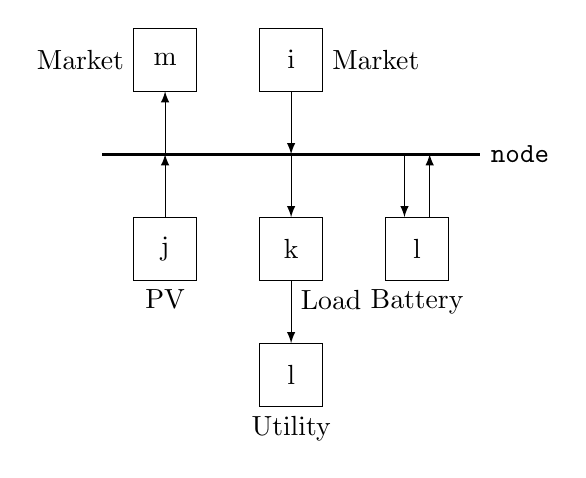
\begin{tikzpicture}[scale=0.8]
        %PV
        \draw (-2.5,0) rectangle node {j} (-1.5,1);
        \node at (-2,0) [anchor = north] {PV};
         \draw[-latex] (-2,1) -- (-2,2);
        %Load
        \draw (-.5,0) rectangle node {k} (.5,1);
        \node at (0,.0) [anchor = north west] {Load};
        \draw[-latex] (0,2) -- (0,1);
        % Battery        
        \draw (1.5,0) rectangle node {l} (2.5,1);
        \node at (2,0) [anchor = north] {Battery};
           \draw[-latex] (2.2,1) -- (2.2,2);
         \draw[latex-] (1.8,1) -- (1.8,2);
        % Utility
        \draw (-.5,-2) rectangle node {l} (.5,-1);
        \node at (0,-2) [anchor = north] {Utility};
        \draw[-latex] (0,0) -- (0,-1);
        % Node
        \draw[very thick, font = \ttfamily] (-3,2) -- (3,2) node [right] {node};
        % Market
        \draw[-latex] (0,3) -- (0,2);
        \draw (-.5,3) rectangle node {i} (.5,4);
        \node at (.5,3.5) [anchor = west] {Market};  
        % Market sell
        \draw[-latex] (-2,2) -- (-2,3);
        \draw (-2.5,3) rectangle node {m} (-1.5,4);
        \node at (-2.5,3.5) [anchor = east] {Market};  
    \end{tikzpicture}
    \caption{More complex system that both buy en sell energy in an energy market, while placing some utility/value on the load (which will then be curtailed if the energy price is too high).}
    \label{fig:sys3}
\end{figure}

%The basic concept of the model is a set of connected \emph{resources} that can exchange energy. A resource is a very general concept and need not represent a physical entitiy. It could for example represent a load profile and enforce the constraint that a certain power flows through it. The resources are connected to \emph{markets} where they buy or sell energy at a certain price. 

This can be extended \textit{ad infinitum} with any number of resources (of different types and parameters) and any number of separate nodes (until limited computing resources kicks in). However, the main feature of the framework is perhaps that the resources may be \textit{aggregated} in \emph{groups} and that these groups can participate in both capacity and activation markets. This is illustrated in figure \ref{fig:groups}. Each resource defines an available capacity and energy activation for balancing (depending on state and properties of the resource). These are then aggregated by the group and the optimization algorithm determines how much to sell into each market.

\begin{figure}
    \centering
    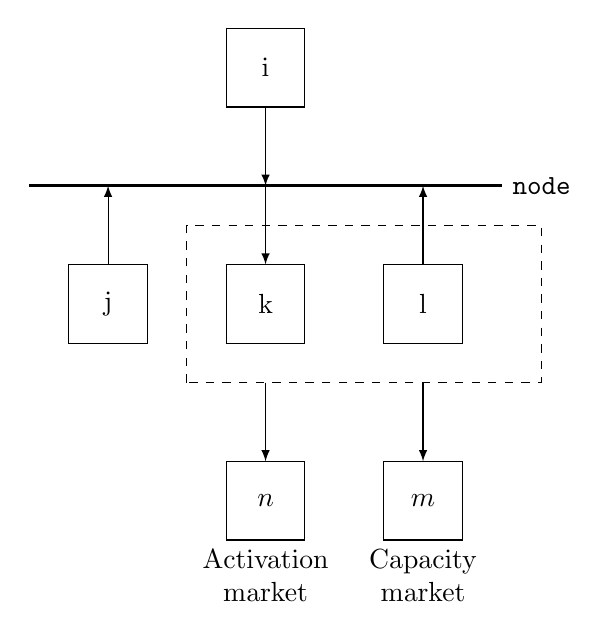
\begin{tikzpicture}
        %PV
        \draw (-2.5,0) rectangle node {j} (-1.5,1);
         \draw[-latex] (-2,1) -- (-2,2);
        %Load
        \draw (-.5,0) rectangle node {k} (.5,1);
        \draw[-latex] (0,2) -- (0,1);
        % Battery        
        \draw (1.5,0) rectangle node {l} (2.5,1);
         \draw[-latex] (2,1) -- (2,2);
        % Node
        \draw[very thick, font = \ttfamily] (-3,2) -- (3,2) node [right] {node};
        \draw[-latex] (0,3) -- (0,2);
        \draw (-.5,3) rectangle node {i} (.5,4);
        %group
        \draw[dashed] (-1,-.5) rectangle (3.5,1.5);
        % Capacity market
        \draw (1.5, -2.5) rectangle node {$m$} (2.5, -1.5) ;
        \draw[-latex] (2,-0.5) -- (2, -1.5);
        \node at (2,-2.5) [anchor = north, align=center] {Capacity \\ market};
        % Activation market
        \draw (-.5, -2.5) rectangle node {$n$} (.5, -1.5) ;
        \draw[-latex] (0,-0.5) -- (0, -1.5);
        \node at (0,-2.5) [anchor = north, align=center] {Activation \\ market};
    \end{tikzpicture}
    \caption{Resources may be aggregated into groups that participate in balancing markets. The resources may participate in multiple balancing at the same time. Some activation and capacity markets are also linked and require participation in both.}
    \label{fig:groups}
\end{figure}

How the system keeps track of the energy during activation may be conceptually somewhat tricky. The value of the power flow (i.e. the value of this variable in the program) to the connected component is not modified and can be thought of as representing the planned (balanced) energy consumption that flows through the component. The real, physical flow will of course change and the activated energy for a given resource must be taken into constraints that account for physical aspects of the resource such as maximum power flows, storage and energy conservation. For example, if a resource is activated in an up-regulation market, the actual flow of energy into the node will be planned flow minus the activated energy. 

Furthermore, note that the activated energy supplied from a particular resource is not tied to reserved capacity from this unit. The group (aggregator) collects the required activation based on all position in capacity markets (or direction participation) in activation markets and divides this optimally between the various resources. Thus for each resource there is no enforced constraint between the reserved capacity and the activation, only that they are within whatever physical constraints that are imposed by the particular resource.

An important feature of the group concept is that it represents an aggregation of resources that are pre-qualified to participate in particular balancing markets. A resource may be part of multiple groups (and the optimization algorithm will decide on where to route the balancing capacity) and the groups may extend across resources connected to multiple nodes as long as the nodes are physically part of the bidding area for the particular market. This is illustrated in  figure \ref{fig:multiplenodes}.

\begin{figure}
    
    \centering
    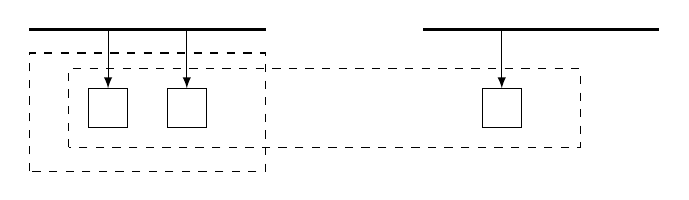
\begin{tikzpicture}[
        comp/.style = {draw, minimum width = .5cm, minimum height = .5cm}
    ]
        \draw[very thick](0,0) -- (3,0);
        \draw[very thick] (5,0) -- (8,0);
        \node[comp] at (1,-1) {} ;
        \node[comp] at (2,-1) {} ;
        \node[comp] at (6,-1) {} ;
        \draw[-latex] (1,0) -- (1,-0.75);
        \draw[-latex] (2,0) -- (2,-0.75);
        \draw[-latex] (6,0) -- (6,-0.75);
        \draw[dashed] (.5,-1.5) rectangle (7,-.5);
        \draw[dashed] (0,-1.8) rectangle (3,-.3);
    \end{tikzpicture}
    \caption{Groups may aggregate resources across multiple nodes and a single resource may be part of multiple groups.}
    \label{fig:multiplenodes}
\end{figure}

Even though the framework is primarily an energy market framework, it is possible to place a \emph{grid} component between the node and the energy markets that represent physical limitations and possible costs (tariffs) of the grid connection that may be fixed or function of the power flow. The cost function may in theory be arbitrarily complex but will quickly result in nonlinear or non-convex models that will put additional demands on the solver used.

The sum up, the different types of components used in the model are

\begin{itemize}
    \item Markets
    \item Nodes
    \item Resources (load/generation and storage)
    \item Grids
\end{itemize}

In addition, the framework utilize the following to concepts to connect and aggregate components

\begin{itemize}
    \item Groups 
    \item Connections
\end{itemize}

For each of the component types in the list, a library of particular components with different properties are provided. The different particular components within each category and their mathematical description are described in the following sections.

A final object in the software to mention is a TimeStruct object. This merely defines the number of the time steps and their units. 

\section{Sets}

Before moving on to describe the components we will introduce a few \emph{sets} that will facilitate the mathematical description of the components.

\begin{itemize}
    \item [$\resources$] The set of all resources.
    \item [$\markets$] The set of all markets.
    \item [$\groups$] The set of all groups.
\end{itemize}

It is also useful to describe a few subsets,

\begin{itemize}
    \item [$\resourcesg$] The set of all resources contained in group $g$ \footnote{E.g. in fig. \ref{fig:groups} if we denote the group by $g$ then $R_g = \{k,l\}$.}.
    \item [$\marketsg$] is the set of all markets connected to group $g$. \footnote{See fig. \ref{fig:groups} where multiple balancing markets are connected to the same group.}
    \item [$\resourcesn$] is the set of all resources connected to node $n$.\footnote{E.g. for fig \ref{fig:groups} $\resourcesn = \{j,k.l\}$.}
    \item [$\groupsr$] The set off all groups to which resource $r$ belongs.
    %\item [$\componentsr$] The set of all entities (resources, groups, markets) connected to resource $r$
    \item [$\inputs_i$] The set components that transmit power to component $i$. 
    \item [$\outputs_i$] The set components that receive power from component $i$.
\end{itemize}

%$\resourcesg$ is the set of all resources contained in group $g$. E.g. in fig. \ref{fig:groups} if we denote the group by $g$ then $R_g = \{k,l\}$. We can also see in the same figure that multiple balancing markets may be connected to the same group. $\marketsg$ is the set of all markets connected to group $g$. $\resourcesn$ is the set of all resources connected to node $n$. E.g. for fig \ref{fig:groups} $\resourcesn = \{j,k.l\}$.

%The various entities are connected to each other. A\emph{connection} implies possible transfer of energy or balancing capacity. 
%We define the following subsets: $\resourcesg$ is the set of all resources connected to group $g$, 
%$\marketsg$ is the set of all markets connected to group $g$,  
%$\resourcesr$ is the set of all resources connected to resource $r$, 
%$\marketsr$ is the set of all markets connected to resource $r$, $\groupsr$ is the set off all groups to which resource $r$ belongs, and $\componentsr$ is the set of all entities (resources, groups, markets) connected to resource $r$

%$\inputs_i$ and $\outputs_i$ are the set of input and output components that resource $i$ transmit power from and to, respectively.

Finally, 

\begin{itemize}
    \item [$\timesteps$] The set of time steps.
\end{itemize}



\newpage

\chapter{Library of concrete components}

This chapter describes the mathematical equations that are implemented in the software for each component. The description for each component is organized as a description of the \emph{parameters}, \emph{variables}, \emph{constraints}, and \emph{objective function terms} they provide to the optimization problem. We will also sometimes use the term \textit{helper variable}. They are variables which are functions of the actual variables in the optimization problem. They are not themselves variables in the optimization model and are just used to simplify notation (and/or coding).

Before starting the description of each resource, let us point out some common nomenclature and concepts that will facilitate reading.

All connections between resources are one-way, i.e. can only transmit energy in one direction. If bi-directional flow is needed, two connections are defined. The direction of power flow is given by the order of the indicies. A power flow from resource $i$ to resource $j$ is denoted by $p_{ij}$ while a power flow from $j$ to $i$ is denoted by $p_{ji}$

Resources may be able to provide balancing capacity. We denote by $r_{it}$ the reserved balancing capacity that may be provided by a resource $i \in \resources$ in time period $t \in \timesteps$. Note that $r_{it}$ denotes the maximum capability of the resource to provide balancing capacity, not what is actually sold to a balancing market. $r_{it}$ will typically depend on both static properties and the dynamic state (value of other variables) of the resource. Unless otherwise specificed the capacity is assumed to be symmetric for up and down regulation. If up and down regulation needs to be distinguished this is denoted by $r^{\uparrow}_{it}$ and $r^{\downarrow}_{it}$, respetively. Simliar notation is used for activation, which we denote by $a_{it}$.

We denote maximum and minimum values by bars over and under the quantity respectively, e.g. $\overline{A}$, \underbar{$A$}

Lowercase letters are usually variables while uppercase letters usually used for parameters. Curly uppercase is used for sets as indicated above.

It should also be noted that in a typical implementation, nodes are the only component with multiple input and outputs. Other resources have one input and one output. However (to allow for future extensions) all components are implemented with the option for multiple inputs and outputs and these are referred to by the sets $\outputs_i$ and $\inputs_i$ in the mathematical description. The multiple input/output option has not been tested. This might lead to some confusion. It might be easier for visualization of typical implementations to think of the input and output sets to have a single element for all components other than nodes.

\newpage
\section{Nodes}
\subsection{StandardNode}
A node $i$ represents a lossless distribution of energy among other components. 

\subsubsection*{Parameters}
A node has no parameters
\subsubsection*{Variables}
A node introduces a set of variables $p_{ijt}$ that is the power flowing from node $i$ to component $j \in \outputs_i$ (note that variable for power flowing to node $i$ from component $k$, $p_{ki}$ is defined by component $k$). 

\begin{itemize}
    \item [$p_{ijt}$] Power flowing from node $i$ to component $j$ in time period $t$.
\end{itemize}

\subsubsection*{Constraints}
The component ensures that the net power flow into any node $i$ is zero,

\begin{equation}
    \sum_{j \in \outputs_i} p_{ijt} - \sum_{j \in \inputs_i} p_{jit} = 0 \quad \forall \quad t \in \timesteps
\end{equation}

\subsubsection*{Objective function}
A node adds no terms to the objecive function.

\newpage
\section{Resources}
\label{sect:resources}

\subsection{SimpleCharger}
This resource is characterized by an upper limit on the power output. It may be interpreted as an EV charger that has an upper limit on the charging capacity.%, including power that is routed to other resources.

\subsubsection*{Parameters}

\begin{itemize}
    \item [$\pmax_i$] Maximum power from the charger .
\end{itemize}

\subsubsection*{Variables}
Let the resource be denoted by the index $i$ and outgoing power be connected to a set $\outputs_i$ of target components (both markets and other resources). The resources defines a set of variables 

\begin{equation}
    p_{ijt} \quad \forall \quad j \in \outputs_i \quad t \in \timesteps
\end{equation}

Provided that the resource is part of a group $g$, the resource also defines a set of variables 

\begin{align}
    r^{\uparrow}_{igt} \quad \forall \quad t \in \timesteps, g \in \groups_i \\
    r^{\downarrow}_{igt} \quad \forall \quad t \in \timesteps, g \in \groups_i
\end{align}

that represent the up and down regulation capacity, respectively that is made available to group $g$. We also define the helper variables $r_{it}$ that is the total capacity available from the resource (to be shared among the groups)

\begin{align}
    r^{\uparrow}_{it} \quad \forall \quad t \in \timesteps \\
    r^{\downarrow}_{it} \quad \forall \quad t \in \timesteps
\end{align}

In addition, the resource defines the variables

\begin{align}
    a^{\uparrow}_{igt} \quad \forall \quad t \in \timesteps, g \in \groups_i \\
    a^{\downarrow}_{igt} \quad \forall \quad t \in \timesteps, g \in \groups_i
\end{align}

which are the activated energies from the resource.

\subsubsection*{Constraints}
The net power flow through the charger must be balanced. Let $\inputs_i$ 
and $\outputs_i$ be the set of input and output components connected to the resource, respectively. We impose the constraint

\begin{equation}
    \label{const:simplecharger-energybalance}
    \sum_{j \in \outputs_i} p_{ij} - \sum_{j \in \inputs} p_{ji} = 0
\end{equation}

(note that this is the planned consumption. Any activation by balancing markets will change the real, physical flow of each of these sum by the same amount.)

The activated down-regulation is limited by the possible increase in output power.

\begin{equation}
    \sum_{g \in \groups_i}\adown_{igt} \leq \pmax_i - \sum_{j \in \outputs_i} p_{ijt}
\end{equation}

Note that this equation simulatenously enforces that $\sum_{j \in \outputs_i} p_{ijt} \leq \pmax_i$ since  $\adown_{igt} \geq 0$.

Similarly for up-activation,

\begin{equation}
    \sum_{g \in \groups_i}\aup_{igt} \leq \sum_{j \in \outputs_i} p_{ijt}
\end{equation}

A point which might be worthwhile to note is that up- and down- regulation appear in separate equations. This avoids a rather strange behavior where one could have (planned) output higher than maximum power if one could a priori assume an activated up-regulation (reduced power). This beviour could occur if the net activation was used in the above equations
\footnote{One could perhaps be tempted to use the following relation which potentially could results in the described behavior,
\begin{equation}
    0 \leq \sum_{j \in \outputs_i} p_{ij} + \sum_{g \in \groups_i} \left(\adown_{igt} - \aup_{igt}\right) \leq \pmax_i
\end{equation}
}

Let $\outputs_i$ be the set of output components connected to the resource %\footnote{Seperating external from internal outputs is important so as not to count curtailable power flows multiple times. A more precise definition and method of implementation needs to be designed however.} 
The maximum \emph{possible} up-regulation is limited by the current output,

\begin{equation}
    \label{eq:charger-up-capacity}
    r^{\uparrow}_{it} = \sum_{j \in \outputs_i} p_{ij}
\end{equation}

The maximum down regulation is limited by the difference between the maximum power and the current power output

\begin{equation}
    \label{eq:charger-down-capacity}
    r^{\downarrow}_{it} = \pmax_i - \sum_{j \in \outputs_i} p_{ij}
\end{equation}

A resource may be connected to multiple groups (i.e. have the technical capabilities to participate in multiple markets) and the balancing capacity must then be shared among the groups. Let $r_{gt}$ be the capacity available from group $g$ (this variable is defined in the \textit{group} component, see sect. \ref{sect:groups}).
\footnote{Not yet implemented in code as only one group and one market has been defined so far.}% 
The resource thus sets

\begin{align}
    \sum_{g \in \groups_i} \rup_{igt} &= \rup_{it} \\
    \sum_{g \in \groups_i} \rdown_{igt} &= \rup_{it}
\end{align}

Note, that these constraints are only in set if the resource is part of at least one group. Otherwise \ref{eq:charger-down-capacity} and \ref{eq:charger-up-capacity} would both be constrained to be zero and the model would have no feasible solutions.

Similarly for activation,

\begin{align}
    \sum_{g \in \groups_i} \aup_{igt} &= \aup_{it} \\
    \sum_{g \in \groups_i} \adown_{igt} &= \adown_{it}
\end{align}

\subsubsection*{Objective function}
Simple charger does not add any terms to the objective function. 

\subsection{Simple Battery}
Simple battery represents an idealized battery where the only physical limitations are the charge capacity and the maximum charging and discharging rates.

\subsubsection*{Parameters}
\begin{itemize}
    \item [$\socmax$] Maximum capacity
    \item [$\pcmax$] Maximum charging rate
    \item [$\pdmax$] Maximum discharging rate
    \item [$Q_0$] Initial state of charge 
\end{itemize}

\subsubsection*{Variables}
Let $\outputs$ be the set of output connections connected to the resource. The resource $i$ defines a set of variables that represent the output from the battery for all time stes

\begin{equation}
    p_{ijt} \quad \forall \quad j \in \outputs, t \in \timesteps
\end{equation}

The resource also defines the variables 

\begin{equation}
    \soc_{it} \forall \quad t \in \timesteps
\end{equation}

that represent the current state of charge of the battery in time step $t$.

The resource defines the variables (provided that the resource is part of a group).

\begin{align}
    r^{\uparrow}_{igt} \quad \forall \quad t \in \timesteps , g \in \groups_i \\
    r^{\downarrow}_{igt} \quad \forall \quad t \in \timesteps , g \in \groups_i
\end{align}

which is the share of the available capacity that may be used in group $g$ that contain the battery $i$ ($g \in \groups_i$).

We also introduce the total capacity available from the battery as a helper variable

\begin{align}
\begin{split}    
    \label{eq:simplebattery:total_r}
    r^{\uparrow}_{it} = \sum_{g \in \groups_i} r^{\uparrow}_{igt} \quad \forall \quad t \in \timesteps \\
    r^{\downarrow}_{it} = \sum_{g \in \groups_i} r^{\uparrow}_{igt} \quad \forall \quad t \in \timesteps
\end{split}
\end{align}

In addition, the resource defines the variables

\begin{align}
    a^{\uparrow}_{igt} \quad \forall \quad t \in \timesteps, g \in \groups_i \\
    a^{\downarrow}_{igt} \quad \forall \quad t \in \timesteps, g \in \groups_i
\end{align}

that represent the up- and down-regulated activated energy, respectively from resource $i$ to group $g$.

\subsubsection*{Constraints}
The net power flow through the battery must be balanced by the change in state of charge. Let $\inputs_i$ and $\outputs_i$ be the set of input and output resources or markets connected to the resource, respectively. We then impose the constraint
\footnote{The software implementation should issue a warning if the battery simultaneously recieves and sends energy or is simultaneously up and down regulated as this would indicate that something is wrong with the model.}

\begin{equation}
    \label{eq:battery-energy-balance}
    \soc_{i,t+1} = \soc_{it} - \sum_{j \in \outputs_i} p_{ijt} + \sum_{j \in \inputs_i} p_{jit} + \sum_{g \in \resourcesg} (\adown_{igt} - \aup_{igt})
\end{equation}

We also have

\begin{equation}
    \soc_{i1} = \socinit
\end{equation}

where $\socinit$ is the inital charge of the battery.

The state of charge may not exceed the maximum capacity $\socmax$,

\begin{align}
    \soc_{it} &\leq \socmax \quad \forall \quad t \in \timesteps \\
    %\soc_{it} &\geq \socmin \quad \forall \quad t \in \timesteps
\end{align}

%$\socmin$

For the last time step $t_f$ we must also ensure that we do not exceed energy limits (state of charge) due to energy flows in the last time step.

\begin{equation}
    \soc_{it_f} - \sum_{j \in \outputs} p_{ijt_f} + \sum_{j \in \inputs} p_{jit_f} + \sum_{g \in \resourcesg} (\adown_{igt} - \aup_{igt})\leq \socmax
\end{equation}

\begin{equation}
    \soc_{it_f} - \sum_{j \in \outputs} p_{ijt_f} + \sum_{j \in \inputs} p_{jit_f} + \sum_{g \in \resourcesg} (\adown_{igt} - \aup_{igt}) \geq 0
\end{equation}


$\pcmax$ and $\pdmax$ are the maximum charging and discharging power from the battery. The resource thus impose,

\begin{align}
    \sum_{j \in \outputs} p_{ijt} + \sum_{g \in \groups_i} \aup_{igt} &\leq \pdmax \\
    \sum_{j \in \inputs} p_{jit} + \sum_{g \in \groups_i} \adown_{igt} &\leq \pcmax
\end{align}

This equation ensures both that the planned power flow does not exceed limits and that any activation will reduce this limit and itself also be limited (does this sentence make it clearer?)

The battery can participate in capacity markets. The total up-regulation $\rup_{it}$ capacity is limited by

\begin{equation}
    \label{eq:up-capacity-battery}
    \rup_{it} = \pmax^D + \sum_{j \in \inputs} p_{jit}- \sum_{j \in \outputs} p_{ijt}
\end{equation}

While the down-regulation capacity $\rdown$ is limited by

\begin{equation}
    \label{eq:down-capacity-battery}
    \rdown_{it} = \pcmax -   \sum_{j \in \inputs} p_{jit}+ \sum_{j \in \outputs} p_{ijt}
\end{equation}

Recall here that $r_{it}$ (both up and down) is just a helper variable defined by eqs. \ref{eq:simplebattery:total_r}.

\begin{equation}
    \label{eq:resource-groups}
    r_{it} = \sum_{g \in \groups_i} r_{igt}
\end{equation}

In addition we cannot reserve capacity that if activated would lead to a state of charge which is outside limits,

\begin{equation}
    \soc_{it} - \sum_{j \in \outputs} p_{ijt} + \sum_{j \in \inputs} p_{jit} + \sum_{g \in \resourcesg} (\rdown_{igt} )\leq \socmax
\end{equation}

\begin{equation}
    \soc_{it} - \sum_{j \in \outputs} p_{ijt} + \sum_{j \in \inputs} p_{jit}  \sum_{g \in \resourcesg} ( \rup_{igt}) \geq 0
\end{equation}

Note that only one direction for capacity enters in these equations. Thus we consider a worst-case scenario and avoid that a combination of up and down regulation can satisfy these equations

Also note that the last constraints \ref{eq:down-capacity-battery} and \ref{eq:up-capacity-battery} are only set if the battery is part of any group, otherwise there would be no feasible solutions to these two equations.

%Similarly,

%\begin{equation}
%    \label{eq:resource-groups}
%    a_{it} = \sum_{a \in \groups_i} a_{igt}
%\end{equation}

\newpage
\subsection{StandardBattery}

[IN PREPARATION]

\subsubsection*{Parameters}


\subsubsection*{Variables}
\subsubsection*{Constraints}
\subsubsection*{Objective function}

\newpage
\subsection{Electric vehicle}
[IN PREPARATION]
This resource represents the battery in an electrical vehicle which is connected to the node only in specific time steps.

\subsubsection*{Parameters}

\begin{itemize}
    \item [$\socmax_i$] Battery maximum energy capacity
    \item [$\ub{R}$] Maximum allowed fraction of capacity
    \item [$\lb{R}$] Minimum allowed fraction of capacity
    \item [$\eta^C$] Charging efficiency
    \item [$\eta^D$] Discharging efficiency
    \item [$\xi^D$] Internal discharge rate
    \item [$t_a$] Arrival times
    \item [$t_d$] Departure times
    \item [$\lb{R}_0$] Fraction of capacity at arrival times.
    \item [$\lb{R}_A$] Minimum allowed fraction of capacity at departure times.
\end{itemize}
\subsubsection*{Variables}
The resource introduces the following variables.

$q_i$ is the current state of charge. $p_{ij}$ is the power flowing from  EV $i$ to  node $j$ (The power into the battery is introduced by the connected node)

Introduce the set $T'$ of timepoints such that for any $t \in T'$

\begin{equation}
    t_a^k\leq t \leq t_d^k
\end{equation}

where $t_a^k$ and $t_d^k$ are the kth arrival and departure time.

\subsubsection*{Constraints}
The resource introduces the following constraints.

The state of charge $q_i$ is bound by

\begin{equation}
    \lb{R}_i \socmin_i \leq \soc_{it} \leq \ub{R}_i\socmax_i  \quad \forall t \in T'
\end{equation}

The state of charge in the next time step is given by

\begin{equation}
    \soc_{i,t+1} = (1-\xi^D)\soc_{it} + \eta^C p_{jit} - \frac{1}{\eta^D}p_{ijt}
\end{equation}

(end conditions...)

\subsubsection*{Objective function}
The resource introduces no terms to the objective function

\newpage

\subsection{Fixed Load}
This component represents a required and fixed load that must be drawn from the system at every time step. The require power may vary from time step to time step. This represents load that cannot be curtailed, i.e. has infinite value for the user. 

\subsubsection{Parameters}
A fixed load $j$ has a parameter $P_{jt}$ which is the required power flowing to the fixed load $j$ in time step $t$.

\begin{itemize}
    \item [$P_{jt}$] Required load
\end{itemize}

\subsubsection{Variables}
No variables introduced

\subsubsection{Constriants}
The fixed load $j$ introduces the constraint the the power drawn from the connected node $i$, $p_{ijt}$ is equal to $P_{jt}$

\begin{equation}
    p_{ijt} = P_{jt}
\end{equation}

\subsubsection{Objective function}
No terms introduced.

\newpage
\subsection{Variable Load}
This resource $j$ represents a load which is limited by an upper and lower bound. Each bound can be a single value or a time series, and either bound can be made redundant by setting to $\infty$ or zero, respectively.

The load has a single input connected to node $i$ and possibly a single output connected to a market (e.g. a utility) $k$ that represents the value placed on the energy by the load.

\subsubsection*{Parameters}
\begin{itemize}
    \item Upper bound $\ub{P}_{jt}$
    \item Lower bound $\lb{P}_{jt}$
\end{itemize}

\subsubsection*{Variables}
This resource introduces a new helper variable $p_{jkt}$ which is the output power that (possibly) flow to a market component if such a component is connected to the load.

\begin{itemize}
    \item [$p_{jkt}$] Output power
\end{itemize}

\subsubsection*{Constraints}
The power is limited by upper and lower bounds

\begin{align}
    p_{ijt} &\leq \ub{P}_{jt} \\
    p_{ijt} &\geq \lb{P}_{jt} 
\end{align}

where $p_{ijt}$ is the power flowing to the load $j$ form the connected node $i$.

The incoming power must be balanced by the outgoing power if connected,

\begin{equation}
    p_{ijt} = p_{jkt} \quad \forall t \in \timesteps
\end{equation}

\subsubsection*{Objective function}

No contribution to objective function.

\subsection{Integrated Load}

\subsection{LinearTariff}

This component simulates a grid tariff that is proportional to the power flowing on a line. The constant of proportionality can be constant or vary with time. The component also supports an upper bound on the power flowing through the component (from the grid) that potentially vary with time (e.g. by DSO curtailment).

\subsubsection{Parameters}

\begin{itemize}
    \item [$C_t$] price per unit of power flowing through the component. 
    \item [$\ub{P_t}$] An optional upper bound on the power flowing through the component. May vary from time step to time step.
\end{itemize}

\subsubsection{Variables}

\begin{itemize}
    \item [$p_{ijt}$] Power flowing from this component $i$ to a connected component $j$
\end{itemize}

\subsubsection{Constraints}
    The power flowing from this component $j$ to a component $k$ must be equal to the power $p_{ijt}$ flowing to the component from a source $i$

    \begin{equation}
        p_{ijt} = p_{jkt}
    \end{equation}

    In addition if an upper bound is set we have

    \begin{equation}
        p_{jkt} \leq \ub{P_t}
    \end{equation}

\subsubsection{Objective function}

The grid tariff is added as term $z_j$ to the objective function as 

\begin{align}
    z_j = \sum_t C_t p_{jkt}
\end{align}

\newpage
\subsection{StepTariff}
This tariff includes a proportional term as in LinearTariff but also an optional tariff that is based on the the time step with the highest power flow in a certain time period.

Note that this component requires the inclusion of binary variables that may significantly affect solution times.

\subsubsection{Variables}

\begin{itemize}
    \item [$p_{ijt}$] Power flowing through the device
    \item [$\delta_k$] indicates if a certain tariff threshold has been exceeded.
    \item [$P_k$] Thresholds for bounds. 
    \item [$\ub{P}$] upper bound on the power
\end{itemize}

\subsubsection{Constraints}

The following constraint ensures that $\delta_x = 1$ if 

\begin{equation}
    p_{ijt}-P_k \leq \ub{P}\delta_k \forall k,t
\end{equation}




\newpage
\section{Groups}
\label{sect:groups}

A \emph{group} is a collection of resources. The group aggregates the the potential of the resources to provide balancing capacity or activation and can sell this to balancing markets connected to the group.  An important conceptual idea behind the group is that it aggregates resources with similar technical properties that enable them to participate in a certain subset of balancing markets with corresponding technical demands.

All resources which are part of a group are implicitly assumed to have a connection to the grid where they can transmit activeted power.

\subsubsection*{Variables}

\begin{itemize}
    \item [$\rup_{gt}$] Maximum up regulation capacity (power) the group can sell to the connected markets
    \item [$\rdown_{gt}$] Maximum down regulation capacity (power) the group can sell to the connected markets
    %\item [$a_{gt}$] activation
\end{itemize}

\subsubsection*{Constraints}

\textit{Capacity}

The group aggregates the balancing capacity of the resources in the group to a total available balancing capacity for the group $r_{gt}$. This variable is thus constrained by

\begin{equation}
     r_{gt} = \sum_{i \in \resourcesg} r_{igt}
\end{equation}

where $r_{igt}$ is the available balancing capacity from resource $i$ provided to group $g$. This variable is defined in the individual resources (see sect. \ref{sect:resources}) and constrained by their individual properties and state. The available capacity from a resource is shared among the groups to which it belongs (see e.g. eq. \ref{eq:resource-groups}). 

The same expressions is used for separate up and down regulation, if necessary. Note that resources may only participated in balancing markets through groups
\footnote{This design choice was based on the premise that the main goal of the software is to analyze \emph{aggregation} of  energy resources (hence the name AggregatorX) and simplify code implementation. If the user needs a single resource to participate in a balancing market, one may simply wrap the resource in a group containing only this resource.}

Each group $g$ sells capacity $r_{mt}$ to a market $m$ it is connected to (that is, the markets for which it meets the technical requirements), up to its available capacity,

\begin{equation}
\label{const:rm_lt_rg}
\sum_{m \in \marketsg} r_{mt} \leq r_{gt}
\end{equation}

The variable $r_{mt}$ is defined by the individual markets (see sect. \ref{sect:markets}). Note that a group may connect to multiple markets, while a market may only be connected to a single group. 
\footnote{It is in some sense redundant to have multiple groups and at the same time let each group participate in multiple markets (one could just define more groups and let each group be connected to a single market). This design is (currently) chosen because for some use cases it might be more conceptually simple to group resources according to technical capability (e.g. capable for FCR), but than have this group participate in multiple markets (FCR-N, -D, D-1, D-2...) rather than defining a group for each market.}.


 
\textbf{Activation}

Each balancing market might result in some required activation (activated energy flow), either as a consequence of the provided capacity and resulting activation due to system conditions, or through participation in activation markets. A capacity market might provide a variable $a_{mt}$ which is the required activation due to a position $r_{mt}$ in the capacity market. 

%The group maintains a variable $a_{gmt}$ which is the activated energy transmitted from group $g$ to market $m$. We thus set

%\begin{equation}
%    a_{gmt} = a_{mt} 
%\end{equation}


Each resource maintains a variable $a_{igt}$ which is the activated energy flowing from the resource $i$ to group $g$ (possibly seperate for up and down if relevant). These variables are used in the energy balance of the resource. The group enforces the constraint that 

\begin{equation}
    \label{eq:activation-group-resource}
    \sum_{m \in \marketsg} a_{mt} = \sum_{i \in \resourcesg} a_{igt}
\end{equation}

An implication of this is that any of the resources in the group may be used to supply the activated energy, not necessarily the resource that provided the capacity.

This also implies that the variables of the activation markets must be de defined before the groups have been defined, such that the variable is available.

\subsection{FFRProfil}

Add existing requirement that activation is zero

Add constraint that bid has to be same for all time steps.

\section{Markets}
\label{sect:markets}

A \emph{market} is a component where (activated) energy or reserved capacity is purchased or sold. Each market $m$ has a  property $\sign_m \in \{-1,1\}$ which represents if energy is sold (output) or purchased (input), respectively. This feature is provided so that the system can both buy and sell energy in a particular market (e.g. day-ahead). In general, a market has a predefined price per quantity (energy or capacity) and contributes a set of terms $Z_m$ in the objective function $Z$ , conceptually

\begin{equation}
    Z = \sum_{m \in \markets} Z_m
\end{equation}

and we seek $\max Z$.

\newpage
\subsection{Utility}
This component represent the utility, i.e. the value, attributed to a particular load. If the effective price of energy 
\footnote{By effective, meaning that if e.g. a battery is available energy may possibly have been bought at a lower price than the energy price in current time step, thereby having a lower effective price. There is no precise definition of this term as it depends on the resources and markets available to the system.}
is lower than the utility, the load will typically be maximized within bounds of other constraints otherwise it will be minimized. Other resources and constraints might affect this behaviour.

\subsubsection*{Parameters}

\begin{itemize}
    \item [$C_t$] The utility of the energy, how much we are willing to pay for it.
    \item [$\sigma$] Market \say{direction} (Set $\sigma = -1$ for most scenarios, i.e. we sell energy to this component. $\sigma = 1$ would mean a cost to deliver the energy, which could be relevant where we have to pay to \say{get rid of} some energy (same behavior could be achieved with negative values of $C_t$.
\end{itemize}

\subsubsection*{Variables}
No variables introduced. The connected load determines the power flowing to the utility.

\subsubsection*{Constraints}
No constraints introduced

\subsubsection{Objective function}
The component adds a term to the objective function representing the value of the power flowing through the connected load.

\begin{equation}
    Z_m = -\sigma C_t p_{ijt}
\end{equation}

where $p_{ijt}$ is the power from load $i$ to the utility component $j$.

\newpage
\subsection{SimpleDAMarket}
This component, denoted by $m$, represents a day-ahead market in it's simplest form. Energy can be purchased according to a predefined market price, that is provided as input from the user.

\textbf{Variables}

Each SimpleDAMarket introduces a set of variables $p_{mt}$ with $t \in \timesteps$, that represents the average power purchased from the market in the period $t$. The power is transmitted to a single resource in the model.

\textbf{Constraints}

SimpleDAMarket introduces no constraints

\textbf{Objective function}

The market defines a price for every time unit $C_{mt}$ as a parameter. It contributes with a term

\begin{equation}
    Z_m = -\sum_{t \in \timesteps} \sign_m C_{mt}p_{mt}
\end{equation}

to the objective function

\newpage
\subsection{SimpleMarket}
This component represents an abstract market where energy can be sold according to a predefined price per time unit provided by the user.

\textbf{Variables}

Each SimpleMarket $m$ introduces a set of variables $p_{mt}$ with $t \in \timesteps$, that represents the average power sold in the market in the period $t$. The power is transmitted from a single resource in the model. 

(more on curtailable loads)

\textbf{Constraints}

The power $p_{mt}$ sold to this market must be equal to the power transmitted from the resource connected to it

\begin{equation}
    p_{mt} = p_{imt}
\end{equation}

where $p_{imt}$ is the power transmitted from resource $i$ to market $m$ (note that most equality constraints between variables are redundant, but are used for better conceptual transparency and in some cases, ease of programming. It is assumed that these redundant variables are removed by the presolver and has no effect on the efficiency of the model).

\textbf{Objective function}

The market defines a price for every time unit $C_{mt}$ as a parameter. It contributes with a term

\begin{equation}
    Z_m = -\sum_{t \in \timesteps} \sign_m C_{mt}p_{mt}
\end{equation}

to the objective function

\subsection{FFRProfil}
This market represents Statnetts FFR Profil market. A single price $C$ for reserved capacity is given for a particular set of time units.

\textbf{Variables}

The market introduces a variable $r_{mt}$ that represents the capacity that is reserved to the market.

\textbf{Constraint}

No new constraints are introduced for FFRProfil\footnote{A minimum bid could be a future option} by the market, but a constraint involving $r_{mt}$ is in effect from the group the market is connected trough eq. (\ref{const:rm_lt_rg})

\textbf{Objective function}

FFRProfil introduces the sum of terms $Z_m$ to the objective function

\begin{equation}
    Z_m = -\sum_{t \in \timesteps} \sign_m Cr_{mt} 
\end{equation}

\subsection{FCRN}
(IN PREPARATION)

FCRN Represents a symmetric (both up and down regulation) FCR market such as FCR-N.

A group participating in FCRN must continuously provide activated energy depending on the frequency deviation $\Delta f_t$ in the power system. $\Delta f_t$ represents the frequency deviation from the nominal frequency $f_0$, averaged over the time step $t$, 

\begin{equation}
    \Delta f_t = \frac{1}{T}\sum_{\tau = t}^{t+T} (f(\tau)-f_0) \Delta{\tau}
\end{equation}

where samples $\tau$ ar taken at a much shorter period than $T$
\footnote{Note that the sampling rate used to control activation and the sampling rate used by the system operator for clearing might be different. This issue is not taken into account here. Rules exist regarding these sampling rates.}. $\Delta f_t$ must be provided as input for each timestep of the analyzed period.

\subsubsection*{Parameters}

\begin{itemize}
    \item [$\Delta f_t$] Average frequency deviation.
    \item [$\Delta f^N$] Maximum frequency deviation allowed where the activation is in effect.
    \item [$C_{mt}^R$] Price for capacity reservation.
    \item [$\cupa_{mt}$] Price for activated up regulation.
    \item [$\cdowna_{mt}$] Price for activated down regulation.
\end{itemize}

\subsubsection*{Variables}
The FCRN market $m$ introduces a variable $\rup_{mt}$ and $\rdown_{mt}$ which represents, respectively, the up and down capacity reserved in the FCR market.
\footnote{These are equal as enforced in the constraints below. Two variables are introduced to be compatible with other non-symmetric markets that share the capacity in the individual groups. Having two variables is a programmatic convenience.}

It also introduces the helper variable
\footnote{Note that helper variables are not a new variables introduced in the optimization model, it is simply a variable that is a function of other optimization variable (see eq. \ref{eq:fcr-capacity-activation} below) and introduced to facilitate transparency and programmability.}
$\aup_{mt}$ and $\adown_{mt}$ which represents the activated energy for up and down regulation, respectively. 

\subsubsection{Constraints}
Eq. \ref{const:rm_lt_rg} ensures that the total available balancing capacity from a group to this market is not exceeded.

Since FCRN is symmetric, we require

\begin{equation}
    \rup_{mt} = \rdown_{mt} \quad \forall t \in \timesteps
\end{equation}

From the frequency deviation, two new parameters are calculated

\begin{align}
    \dfdown_t = 
        \begin{cases}
            \Delta f_t & \text{if \, } f_N > \Delta f_t > 0 \\
            0 & \text{if \,} \Delta  f_t \leq 0 \vee \Delta f_t \geq f_N 
        \end{cases} \\
    \dfup_T = 
        \begin{cases}
            \Delta f_t & \text{if \,} -f_N < \Delta f_t < 0 \\
            0 & \text{if \,}\Delta  f_t \geq 0 \vee \Delta f_t \leq -f_N
        \end{cases}
\end{align}

The activated power is set similarly for both up and down regulation to  

\begin{align}
    \label{eq:fcr-capacity-activation}
    \aup_{mt} &= \rup_{mt} \frac{\Delta f_t}{\Delta f^N}  \\
    \adown_{mt} &= \rdown_{mt} \frac{\Delta f_t}{\Delta f^N} 
\end{align}

where $\Delta f^N$ is the maximum frequency deviation allowed within normal operation (typically 0.1 Hz for FCR-N). If $\Delta f_t > \Delta f^N$ the system enters disturbance mode (FCR-D), and $a_{mt} = 0$.

%The activated energy must be balanced by energy flows from the resources in the group. The group maintains the variable $a_{gmt}$ which is the activitated energy from group $g$ to market $m$ so the markets enforce that

%\begin{equation}
%    a_{gmt} = a_{mt}
%\end{equation}
The group the market is connected to enforces constraint \ref{eq:activation-group-resource} such that the activation from the resources in the group meets the demand of this market (and others). The activated energy in the resources enters the constraint in their energy balance (e.g. as in \ref{eq:battery-energy-balance}. % and \ref{const:simplecharger-energybalance}

%The group imposes the restriction that (belongs to groups, me thinks)

%\begin{equation}
%    a_{mt} = \sum_{i \in R_g} a_{it} 
%\end{equation}

%As indicated above (NOT YET), resources checks that activated energy in groups to which they are connected and adds this to their energy balance (e.g. Eq. (\ref{const:simplecharger-energybalance}).

Note also that resources that pariciapte in FCR may not participate in other balancing markets. 

\begin{equation}
    R_g \bigcap \left( \bigcup_{h \in G, h \neq g} R_h \right) = \varnothing
\end{equation}

This is done by checking that the resources in the FCR group are not part of any other group.

\subsubsection{Objective function}
The market adds a term

\begin{equation}
    Z_m^R = \sum_t C^R_{mt} r_{mt}
\end{equation}

to the objective function representing the reserved balancing capacity. $C^R_{mt}$ is the price for FCR-N in time period $t$. In addition there is a term for the activated energy

\begin{align}
    Z_m^A = \cupa_{mt} \aup_{mt} \\
    Z_m^A = \cdowna_{mt} \adown_{mt}
\end{align}

The price for activated FCR-N is typically the same as for RK/mFRR-EAM. If $\Delta f_t > \Delta f^N$ the system enters disturbance mode (FCR-D is activated) and no renumeration is given for FCR-N. 




\end{document}